% Modular adaptation of the supplied ICEIB2027-IEEE starter.
% Overleaf: select main.tex and pdfLaTeX. Compile twice for cross-references.
% Sources: project README (973148b) and accompanying Chinese proposal analysis.
\documentclass[conference]{IEEEtran}
\usepackage{cite}
\usepackage{amsmath,amssymb}
\usepackage{booktabs,tabularx,array}
\usepackage{algorithm,algpseudocode}
\usepackage{tikz}
\usetikzlibrary{arrows.meta}
\usepackage{url}
\newcolumntype{Y}{>{\raggedright\arraybackslash}X}
\tikzset{unit/.style={draw,rounded corners=1.5pt,align=center,inner sep=3pt,
 minimum height=8mm,font=\footnotesize},link/.style={-{Stealth[length=1.6mm]},thin}}
% Replace the three fields below with the confirmed submission details.
\newcommand{\paperauthors}{Author name(s)}
\newcommand{\paperaffiliation}{Department and institution}
\newcommand{\paperemail}{Corresponding author email}
\begin{document}
\title{A Data-Grounded Conversational AI Agent for Integrated Home Environment Assessment and Outdoor Activity Recommendations}
\author{\IEEEauthorblockN{\paperauthors}
\IEEEauthorblockA{\paperaffiliation\\\paperemail}}
\maketitle

\begin{abstract}
A resident deciding where to dry laundry needs to know what the room sensor measured and what weather is expected at the balcony during the drying period. A drop in indoor relative humidity answers neither question on its own. We propose DietSense, a conversational agent that combines room measurements, township forecasts, confirmed appliance operations, and resident feedback. An ESP32 sensor supplies temperature and relative humidity through MQTT. Python routines analyze timestamped records in SQLite, while a language model selects from approved tools and explains their results. A query triggers a check of location, time, and source. Background monitoring groups sustained changes into events and requests confirmation when the answer would affect a recommendation. A planned two-week pilot will compare fixed rules with a shallow decision tree on chronologically held-out events. It will also assess whether access to confirmed context improves the evidence cited in answers enough to justify the questions residents receive. The contribution at this stage is the system design and an event-level evaluation protocol.
\end{abstract}
\begin{IEEEkeywords}
conversational agents, indoor environmental monitoring, Internet of Things, thermal comfort, weather forecasts
\end{IEEEkeywords}

\section{Introduction}\label{sec:intro}
A room sensor and a weather forecast can both report relative humidity for the same afternoon. One describes air near the sensor when it sampled the room. The other describes an expected condition over a future interval at a representative outdoor location. If a resident asks whether laundry will dry on the balcony, the distinction determines which evidence belongs in the answer. If the resident instead asks why the room feels less humid, an operation record or a report of an open window may matter more than the forecast.

Adaptive-comfort research links occupants' preferences to thermal history and context~\cite{deDear}. Taiwan's Central Weather Administration (CWA) provides a separate source of context through forecasts for 368 townships and districts. Its product documentation identifies the representative location and cautions that conditions can vary within a township~\cite{cwa}. A home assistant must therefore resolve two references that are easily implicit in a question: the place the resident means and the interval over which the advice will apply.

The DietSense project addresses three household decisions: interpreting equipment use in one room, planning an outing, and choosing between indoor and outdoor drying~\cite{project}. The design links each factual claim to the observation, forecast period, or confirmation that supports it. A second contribution is a background procedure that merges sustained changes into events and limits repeated requests for feedback. A third is a planned comparison that measures both prediction quality and the cost of gathering extra evidence. Section~\ref{sec:related} identifies assumptions inherited from prior work. Sections~\ref{sec:method} and~\ref{sec:experiments} describe the design and pilot.

\section{Related Work}\label{sec:related}
\subsection{Conversational tools and smart-home data}
ReAct demonstrates how a language model can obtain information by interleaving reasoning with external actions~\cite{react}. AdaHome routes smart-home requests and uses interaction history to handle preference-dependent commands~\cite{adahome}. DietSense adopts the separation between interpreting a request and executing a tool. A preference about drying clothes indoors may guide a recommendation, whereas a statement that the dehumidifier ran requires an operation record or confirmation. Keeping these histories separate allows a resident to correct one without changing the other.

AgentSense generates labeled sensor streams from simulated household activities~\cite{agentsense}. Such streams can support activity-recognition research. In the present setting, the difficult cases are episodes in which several devices operate together or a resident cannot recall what happened. A simulation supplies its own event labels. A home deployment must account for who confirmed an event and when that information became available.

\subsection{Environmental models and the choice of labels}
The CBE Thermal Comfort Tool implements comfort models with explicit environmental and personal inputs~\cite{cbe}. DietSense has a single temperature and humidity sensor. It can report a trend and ask how it felt, but lacks several inputs needed for a full comfort assessment. Likewise, the office dataset studied by Candanedo and Feldheim associates environmental measurements with occupancy~\cite{occupancy}. A successful occupancy prediction would not establish which device was operating. Table~\ref{tab:work} identifies the evidence each source contributes and the question left for the pilot.

\begin{table*}[t]
\caption{Prior work and its applicability to the single-room pilot}
\label{tab:work}\centering\footnotesize
\setlength{\tabcolsep}{3pt}
\begin{tabularx}{\textwidth}{@{}l l Y Y Y Y Y Y@{}}
\toprule
Ref. & Year & Problem & Method & Domain knowledge & Data or input & Contribution & Limit for this task\\
\midrule
\cite{react} & 2023 & Retrieve evidence during a task & Tool-using language model & Interactive reasoning & Question answering and decision tasks & External results inform subsequent actions & Sensor location and time need explicit checks\\
\cite{adahome} & 2026 & Interpret household requests & Local language model and routing & Home preferences & Commands and preference histories & Routes requests by intent & A preference cannot confirm a device state\\
\cite{agentsense} & 2026 & Obtain activity labels & Agent-based simulation & Home activities & Virtual sensor streams & Produces labeled activity sequences & Simulated labels cannot verify a real event\\
\cite{deDear} & 1998 & Explain variation in comfort & Adaptive model & Thermal preference & Field surveys in buildings & Relates context to preferred conditions & A population trend cannot label one episode\\
\cite{occupancy} & 2016 & Estimate occupancy & Statistical learning & Office environment & Sensors and occupancy labels & Predicts whether an office is occupied & Occupancy and appliance use are distinct targets\\
\cite{cbe} & 2020 & Calculate comfort indices & Physical and empirical models & Thermal comfort & Environmental and personal inputs & Makes model assumptions explicit & Some inputs are unmeasured in the pilot\\
\bottomrule
\end{tabularx}
\end{table*}


Table~\ref{tab:capabilities} summarizes the capability scope described above. Not reported means that the capability is not established by the discussion in this draft; it does not imply that the cited system lacks it. DietSense entries describe proposed behavior, not verified implementation.
\begin{table*}[t]
\centering\footnotesize
\caption{Capability scope based on the manuscript's related-work descriptions (not a measured comparison).}
\label{tab:capabilities}
\begin{tabularx}{\textwidth}{@{}l Y Y Y Y@{}}
\toprule
System & External tool or data access & Household context & Environmental evidence & Event confirmation \\
\midrule
ReAct~\cite{react} & External actions & Not reported & Not reported & Not reported \\
AdaHome~\cite{adahome} & Request routing & Preference histories & Not reported & Not reported \\
AgentSense~\cite{agentsense} & Simulated sensor streams & Simulated activities & Virtual sensor readings & Simulation labels \\
CBE Tool~\cite{cbe} & Model inputs & Personal inputs & Comfort-model inputs & Not reported \\
DietSense (proposed) & Approved tools & Resident preferences & Room observations and township forecasts & Resident or operation records; unknown states retained \\
\bottomrule
\end{tabularx}
\end{table*}


\section{Proposed Scheme}\label{sec:method}
\subsection{Evidence available at decision time}
Let $t$ denote the instant a query arrives. Let $I$ denote the interval of interest, which may start after $t$, and let $s$ be the requested township. A forecast record $f$ can describe an instant $\tau\in I$ when
\begin{equation}
s_f=s,\quad t_{\mathrm{issued},f}\leq t,\quad
t_{\mathrm{start},f}\leq\tau<t_{\mathrm{end},f}.
\label{eq:forecast}
\end{equation}
If several records satisfy (\ref{eq:forecast}), the tool selects the most recently issued one available to the system by $t$. A request spanning two forecast periods retains both. An uncovered part of $I$ remains visible in the answer. A trip to a second township changes the forecast lookup even when the indoor sensor stays in the same room.

Indoor observations carry a room identifier, sample time, temperature, and relative humidity. The proposed SQLite records distinguish measurement time from receipt time so a delayed MQTT message can be placed in its event without being treated as a fresh observation. The engine evaluates temperature and relative humidity together. Warming air, for example, can reduce relative humidity even when its water vapor content changes little. A derived dew-point trend may help describe this distinction. Neither trend identifies the appliance responsible.

An operation record stores the device, stated interval, source of confirmation, and time of entry. A later correction supersedes the earlier interpretation while retaining both versions. Multiple active devices can coexist. A missing response leaves the status unknown. A comfort report, a device confirmation, and acceptance of a recommendation are separate fields because they answer different questions.

\subsection{Architecture and tool routing}
Figure~\ref{fig:arch} shows the eight modules. The resident provides the room, activity, or destination (M1). The query interface (M2) extracts the time and place or passes an unresolved reference to the planning agent (M3). Acquisition (M4) receives the ESP32 stream over MQTT, obtains CWA forecasts, and retains confirmations in SQLite. The Python analysis engine (M5) computes trends and event features. Domain rules (M6) specify source scope, required inputs, and when an interpretation needs confirmation. The decision module (M7) selects advice or a question. The interaction module (M8) presents the answer and records feedback.

\begin{figure}[t]
\centering
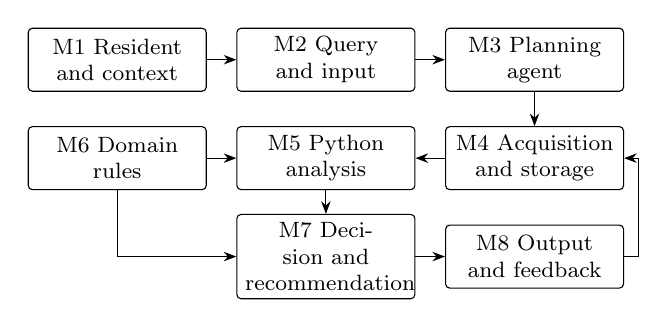
\begin{tikzpicture}[x=1cm,y=1cm]
\node[unit,text width=2.05cm] (user) at (0,0) {M1 Resident\\and context};
\node[unit,text width=2.05cm] (query) at (2.65,0) {M2 Query\\and input};
\node[unit,text width=2.05cm] (agent) at (5.3,0) {M3 Planning\\agent};
\node[unit,text width=2.05cm] (rules) at (0,-1.25) {M6 Domain\\rules};
\node[unit,text width=2.05cm] (analysis) at (2.65,-1.25) {M5 Python\\analysis};
\node[unit,text width=2.05cm] (data) at (5.3,-1.25) {M4 Acquisition\\and storage};
\node[unit,text width=2.05cm] (decision) at (2.65,-2.5) {M7 Decision and\\recommendation};
\node[unit,text width=2.05cm] (out) at (5.3,-2.5) {M8 Output\\and feedback};
\draw[link] (user)--(query); \draw[link] (query)--(agent);
\draw[link] (agent)--(data); \draw[link] (data)--(analysis);
\draw[link] (rules)--(analysis); \draw[link] (analysis)--(decision);
\draw[link] (decision)--(out); \draw[link] (rules.south) |- (decision.west);
\draw[link] (out.east) -- ++(0.18,0) |- (data.east);
\end{tikzpicture}

\caption{A resident query starts at M1. Background monitoring starts at M4 when a sample arrives. Both paths share analytical routines and store subsequent confirmations at M4.}
\label{fig:arch}
\end{figure}

The language model may request a room history, a township forecast, a confirmed operation record, or a deterministic analysis. The requested tool and validated arguments will be logged alongside the returned record identifiers. A numerical change reported in the response must be reproducible from those records. For an outdoor query, the response must attribute future conditions to the forecast and state the applicable interval. A resident can then distinguish a stale source, a wrong destination, and a disagreement about personal preference.

\subsection{On-demand advice and background monitoring}
Figure~\ref{fig:paths} distinguishes two occasions for asking a question. During a resident query, the missing information must matter to the decision at hand. In the background, sustained changes are grouped into one event before the system considers interrupting the resident. Algorithms~\ref{alg:query} and~\ref{alg:monitor} specify how each path handles incomplete evidence.

\begin{figure}[t]
\centering
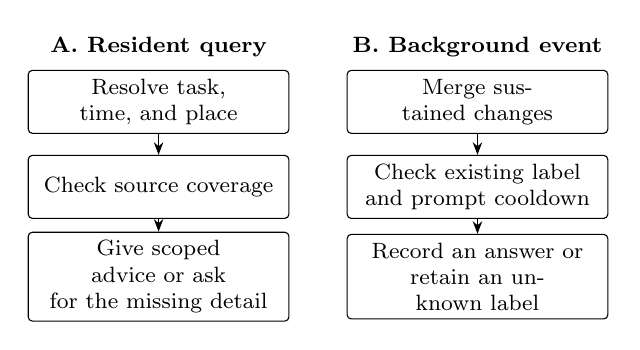
\begin{tikzpicture}[x=1cm,y=1cm]
\node[font=\footnotesize\bfseries] at (0,0) {A. Resident query};
\node[font=\footnotesize\bfseries] at (4.05,0) {B. Background event};
\node[unit,text width=3.1cm] (q) at (0,-0.7) {Resolve task, time, and place};
\node[unit,text width=3.1cm] (m) at (4.05,-0.7) {Merge sustained changes};
\node[unit,text width=3.1cm] (e) at (0,-1.78) {Check source coverage};
\node[unit,text width=3.1cm] (c) at (4.05,-1.78) {Check existing label\\and prompt cooldown};
\node[unit,text width=3.1cm] (a) at (0,-2.92) {Give scoped advice or ask\\for the missing detail};
\node[unit,text width=3.1cm] (r) at (4.05,-2.92) {Record an answer or\\retain an unknown label};
\draw[link] (q)--(e); \draw[link] (e)--(a);
\draw[link] (m)--(c); \draw[link] (c)--(r);
\end{tikzpicture}

\caption{The query may produce a conditional answer immediately. Background monitoring may finish silently when the resident has already been asked.}
\label{fig:paths}
\end{figure}

\begin{algorithm}[t]
\caption{Answer a household query (M1--M8)}\label{alg:query}
\begin{algorithmic}[1]
\Require Query $q$, decision time $t$, available room context
\Ensure Answer with sources, or a targeted clarification
\State Resolve activity, place, and interval (M1--M3)
\If{a required place or interval is ambiguous}
  \State \Return a question identifying the missing detail (M8)
\EndIf
\State Retrieve eligible records with approved tools (M3--M4)
\State Compute trends and check coverage (M5--M6)
\If{a missing fact could change the advice}
  \State Give the supported part and ask for that fact (M7--M8)
\Else
  \State Give advice with source times and scope (M7--M8)
\EndIf
\State Log evidence identifiers and later feedback (M4, M8)
\end{algorithmic}
\end{algorithm}
\begin{algorithm}[t]
\caption{Monitor events and collect feedback (M4--M8)}\label{alg:monitor}
\begin{algorithmic}[1]
\Require Samples, event history, and prompt history
\Ensure Updated event and confirmation status
\State Store the sample and check continuity (M4)
\If{the observation window contains a material gap}
  \State Mark it incomplete and restart the window (M5)
  \State \Return the current evidence status
\EndIf
\State Detect sustained change and merge related windows (M5)
\If{an event needs a label and the cooldown has elapsed}
  \State Ask one question tied to that event (M6--M8)
  \State Record the reply or retain an unknown label (M4, M8)
\EndIf
\State Preserve the event interval and label revisions (M4)
\end{algorithmic}
\end{algorithm}

Consider an illustrative query: \emph{Can I hang the laundry outside for the next two hours?} The agent resolves whether the resident means the home balcony, retrieves the forecast covering that township and interval, and keeps the room reading available if indoor drying is an alternative. If the forecast gives a precipitation probability over a broader interval, the response identifies that interval. A precise rain onset or drying time would require additional evidence. A useful response can still tell the resident which part of the question the forecast covers and whether the indoor alternative has a recent measurement.

\section{Planned Experiments and Discussion}\label{sec:experiments}
\subsection{Pilot collection and reference labels}
The proposed pilot will collect approximately two weeks of single-room observations, operation records, and resident feedback. The evaluation unit for event recognition will be one sustained change episode. Each episode will retain the samples from which its features were computed, the first possible prediction time, and any later confirmation. Each advice query will have a separate record linking the request, tool arguments, evidence, response, and subsequent acceptance or rejection.

For appliance-event evaluation, a confirmed operation log or resident reply will supply the reference label. To accommodate concurrent operations, the proposed scoring scheme treats each tracked device as a separate on/off question. An unconfirmed state remains unscored for that device. Counts of unknown and overlapping states will accompany the scores. A missing reply cannot establish that a device was off. For advice evaluation, a reviewer will compare factual claims with the information actually available when the response was issued.

\subsection{Chronological comparison and ablations}
The fixed-rule baseline will classify events using predeclared conditions on the direction, magnitude, and persistence of temperature and humidity changes. A shallow decision tree will use the same features and training period. Thresholds, tree depth, feature windows, event-merging settings, and cooldown duration will be recorded before evaluating the held-out period. Earlier complete events will be used for development and later complete events for testing. An event crossing the boundary and any overlapping feature windows will be excluded. This grouping addresses temporal dependence between adjacent samples~\cite{roberts}.

The first comparison will use sensor features alone to score both classifiers on identical held-out events. A second comparison will replay the same queries under three conditions: measurements and aligned forecasts alone, the same evidence with previously confirmed device states, and all available evidence with earlier resident preferences. A reply establishing the target state for an event will never serve as an input for predicting that state. Acceptance of a recommendation is likewise available only after the recommendation has been issued. Replay can assess changes in factual consistency and proposed prompts. Acceptance and actual reply rates will be measured only for interactions the resident experienced.

\begin{table}[t]
\centering\footnotesize
\caption{Planned outcomes and their denominators}
\label{tab:metrics}
\begin{tabularx}{\columnwidth}{@{}p{0.28\columnwidth}Y@{}}
\toprule
Outcome & Measurement unit and interpretation\\
\midrule
Event classification & Accuracy on known event--device pairs. Report per-device precision and recall, macro-F1, and class counts.\\
Evidence consistency & Supported factual claims divided by auditable claims. Review source, value, time, and location.\\
Tool correctness & Queries with the required tools and valid arguments divided by audited queries.\\
Acceptance & Accepted recommendations divided by recommendations receiving an explicit judgment. Count unanswered cases separately.\\
Clarification burden & Background prompts per monitored hour, and the fraction of delivered prompts receiving a reply.\\
\bottomrule
\end{tabularx}
\end{table}


\subsection{What the pilot can establish}
Table~\ref{tab:metrics} distinguishes a classifier error from a retrieval error. A tree might recognize an event while the assistant retrieves a forecast for the wrong township. Conversely, the correct forecast and tool sequence can support an answer even when the cause of an indoor change remains unknown. For each device with positive held-out examples, the evaluation will compute its positive-class F1 and average these values across eligible devices. Counts of excluded devices and unconfirmed events will show how much of the deployment the score represents.

Asking after every change could make the labeled subset look unusually easy to classify. The pilot will report monitored hours, candidate events, delivered questions, and replies together. Replay with different cooldown settings can show how many questions each policy would issue. It cannot establish how a resident would have answered a question that was never delivered.

Three failure cases will receive individual review: a sensor reconnects after a gap, two appliances operate during the same event, and the requested destination differs from the home township. Each tests a different decision: whether the system bridges missing samples, whether it forces one cause onto an ambiguous trend, and whether it retrieves the correct forecast. A short single-room study can assess traceability and interaction cost in that setting. Seasonal behavior, unobserved rooms, and the causal effect of an individual appliance remain outside its reach.

\section{Conclusion}\label{sec:conclusion}
DietSense proposes a way to answer household questions while preserving what each source can establish. A room sample describes conditions near one sensor, a township forecast describes an outdoor interval, and a resident confirmation documents a reported action. The prototype design joins those records at query time and leaves unresolved device states visible. The two-week pilot will test how often the agent can substantiate its advice, how often it needs to ask for context, and which event types remain ambiguous. Those observations will guide the decision to extend sensing to additional rooms.


\bibliographystyle{IEEEtran}
\bibliography{references}
\end{document}
